\chapter{Evaluation} % Main chapter title

\label{Chapter4} % For referencing the chapter elsewhere, use \ref{Chapter1} 
\section{Before Testing}
In this Chapter we start the evaluation and testing procedure for the new search algorithm and heuristic. The first step is a preprocessing test, and when the results are analysed, we will start the preliminary tests of the new algorithms. 
\subsection{Preprocessing Test} 
The first thing to do before any tests could be completed was to check all of the IPC domains that would be used in the testing process for any errors. It would also give us a general idea of how long the parsing and encoding would take before the actual search could start. The goal was to remove any domains that had issues or that caused complications for the PDDL4J planner to encode. It would not make the testing environment fair if a domain was unable to be encoded properly and the search algorithm or heuristic ran for a long period of time when no solution would ever be potentially available. 
What we saw was issues with some of the domain files like Barman for example from IPC7. There were other domains like this and we addressed the issues and attempted to generate a new domain file or see if there was a small error inside the file that we could change.
\subsection{Preliminary Test}
In this section, preliminary tests were carried out to see if both the heuristic and the search algorithms were going down the right path to complete the hypothesis. We tested the search algorithm first by running it on the Blocksworld domain from the IPC2 competition. It was tested against the current A* algorithm and the preliminary results showed that the new search algorithms had out-performed A* by a considerable amount. The time for completing all 35 problems was much faster than A*, and also, A* was unable to complete the final 5 Blocksworld problems within the 600 second time limit. 

\begin{figure}[!htb]
    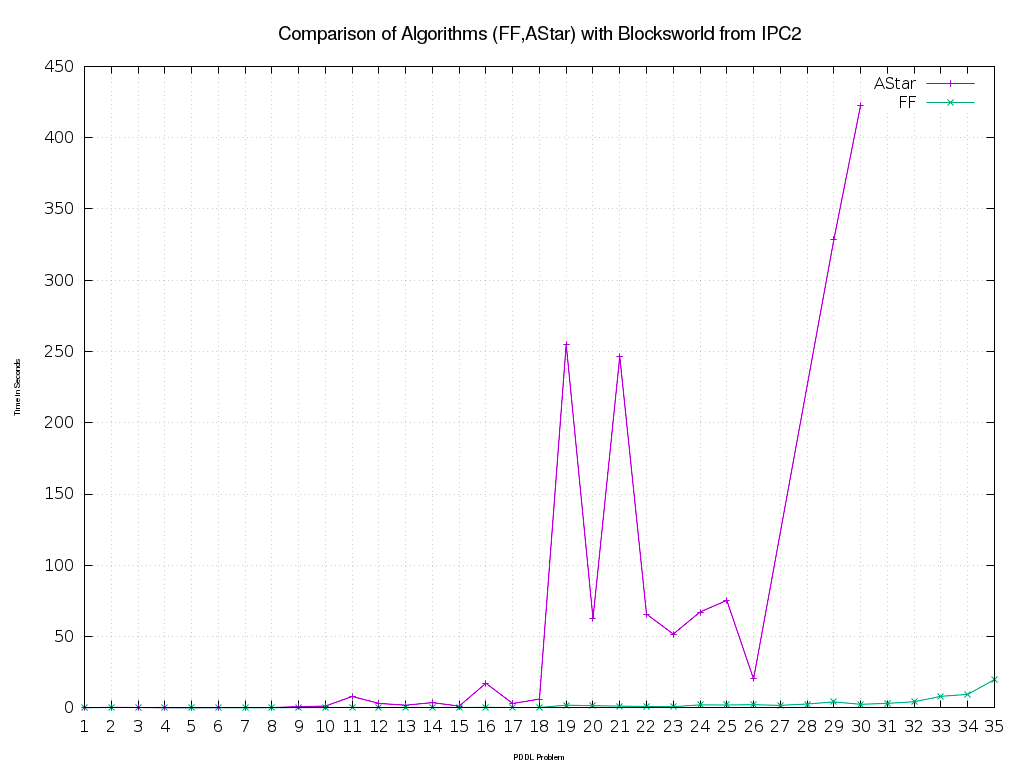
\includegraphics[scale=0.35]{PrelimTestFF.png}
    \caption{Preliminary results on the Blocksworld domain for the new search algorithm vs A*}
    \label{fig:PrelimVsA*}   
\end{figure}

This gave a really good insight to the capabilities of the new algorithm, as well as being on track to prove the hypotheses set out in Chapter \ref{Chapter2}. These results, however, could not be used as they were run on my own computer which does not fit in with the testing environment set out in Chapter \ref{Chapter3}.

The same environment was used to test the $H^m$ heuristic and it was tested on the Mystery domain from IPC1. We tested the new heuristic with Fast Forward and Max to compare the time needed to complete the problems. We achieved good results in that the new heuristic was similar in speed versus Fast Forward for completing the tasks although, as expected, the Max heuristic took longer. 

\begin{figure}[!htb]
    \centering
    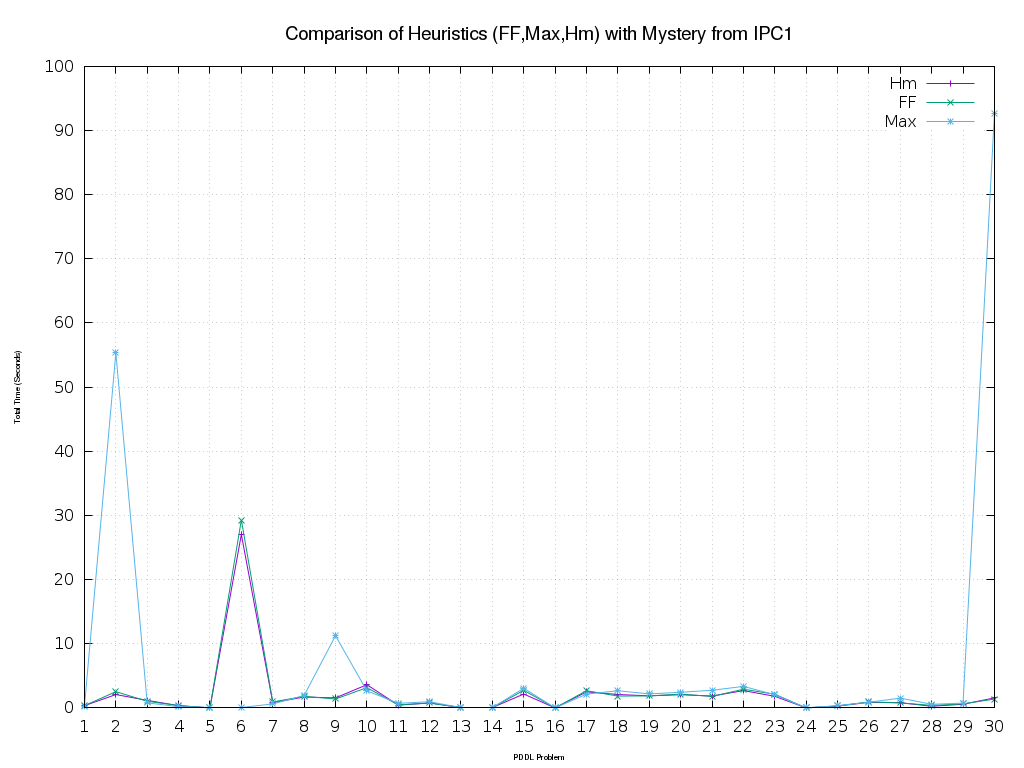
\includegraphics[scale=0.35]{PrelimTestHeuristic.png}
    \caption{Preliminary results on Mystery domain, FF vs Max vs $H^m$}
    \label{fig:PrelimFFvsMaxvsHm}
\end{figure}

There were no differences in plan size and we think this is because the $H^m$ heuristic is admissible \cite{hmAdmissible}, as is Max, so there should not be any differences in the plan length. Also, compared with Fast Forward, all plan lengths were the same. This is possibly due to the Mystery domain being a set of small problems with a small number of objects as well as all the heuristics running with the A* algorithm which should provide optimal plans (with the use of an admissible heuristic). A vigorous testing procedure in the next section should be able to provide the results that we are hoping for.  
\section{A* vs Greedy Best First Search and Enforced Hill Climbing}
As the preprocessing tests and preliminary results showed impressive data for the new search algorithm and heuristic, the testing stage can start against all domains from IPC1-IPC8 as discussed in Chapter \ref{Chapter3}
The table below shows all the domains in which we tested the new algorithm against A*. It also shows the total number of problems within each domain and how many of those problems the planners managed to solve. 
\begin{center}
  \begin{tabular}{ | l | c | r |}
    \hline
    \textbf{Domain} & \textbf{GBFS + EHC} & \textbf{A*} \\ \hline
    Gripper & 20/20 & 7/20 \\ \hline
    Logistics & 0/30 & 7/30 \\ \hline
    Movie & 30/30 & 30/30 \\ \hline
    Mprime & 14/30 & 24/30 \\ \hline
    Mystery & 13/30 & 16/30 \\ \hline
    Blocksworld & 35/35 & 30/35 \\ \hline
    Elevator & 99/99 & 99/99 \\ \hline
    Freecell & 60/60 & 59/60 \\ \hline
    Schedule & 0/100 & 0/100 \\ \hline
    Depots & 15/22 & 16/22 \\ \hline
    Driverlog & 16/20 & 14/20 \\ \hline
    Rover & 0/20 & 2/20 \\ \hline
    Satellite & 14/20 & 12/20 \\ \hline
    Zenotravel & 20/20 & 13/20 \\ \hline
    Airport & 0/50 & 28/50 \\ \hline
    Optical Telegraph & 1/14 & 2/14 \\ \hline
    Philosophers & 10/29 & 5/29 \\ \hline
    Pipesworld & 16/50 & 15/50 \\ \hline
    Psr & 41/50 & 47/50\\ \hline
    Openstacks & 30/30 & 7/30 \\ \hline
    Pathways & 7/30 & 5/30 \\ \hline
    Storage & 17/30 & 15/30 \\ \hline
    Tpp & 15/30 & 7/30 \\ \hline
    Truck & 13/30 & 8/30 \\ \hline
    Pegsol & 29/30 & 27/30 \\ \hline
    Sokoban & 25/30 & 25/30 \\ \hline
    Transport & 0/30 & 0/30 \\ \hline
    Barman & 0/20 & 0/20 \\ \hline
    Nomystery & 7/20 & 13/20 \\ \hline
    Parking & 3/20 & 0/20 \\ \hline
    Childsnack & 2/20 & 0/20 \\ \hline
    Hiking & 0/20 & 0/20 \\ \hline
    Thoughtful & 7/20 & 5/20 \\ \hline
    \textbf{Solved Problems Total} & 559/1089 & 538/1089 \\ \hline
    \textbf{Percentage} & 51.33\% & 49.40\% \\  
    \hline
  \end{tabular}
\end{center}
These are the results for the new algorithm for the PDDL4J planner versus A*. We used the same technique as described in Chapter \ref{Chapter3} to run the tests. A bash script was created so all the domains could be run one after the other and save the results in a text file which was then used to create diagrams with GNUPLOT. We can see some good results from the new search algorithm as well as some strange results, namely from the Rover domain where A* was able to solve only 2 problems out of a possible 20. Then with Airport from IPC4, A* was able to solve 28 out of a possible 50 but GBFS with EHC was unable to solve any of the problems. With Openstacks, GBFS with EHC was able to solve all 30 but A* could only manage 7.
The total number of problems in all of the domains is at the bottom of the table along with the total number of solved problems and the number of problems attempted against problems solved is shown as a percentage. From this we can deduce that GBFS with EHC was able to solve 1.93\% more problems than A*. Even though this is a small percentage, it is still an improvement in regards to the PDDL4J planner and it proves the hypothesis correct. We will now look at some of the problems in detail and explain the findings. All results for the tests are placed in Appendix A at the end of the report. 
\subsection{Graphs and Analysis}
There are many sets of domains that we could choose from but have narrowed it down to 4 in order to demonstrate the difference in time plus memory consumption between the two search algorithms. The domains are Movie from IPC1, Sokoban from IPC6, Blocksworld from IPC2 and Psr from IPC4. The full set will be displayed on GitHub and all information regarding access can be found in Appendix A.
\\
\begin{figure}[!htb]
    \centering
    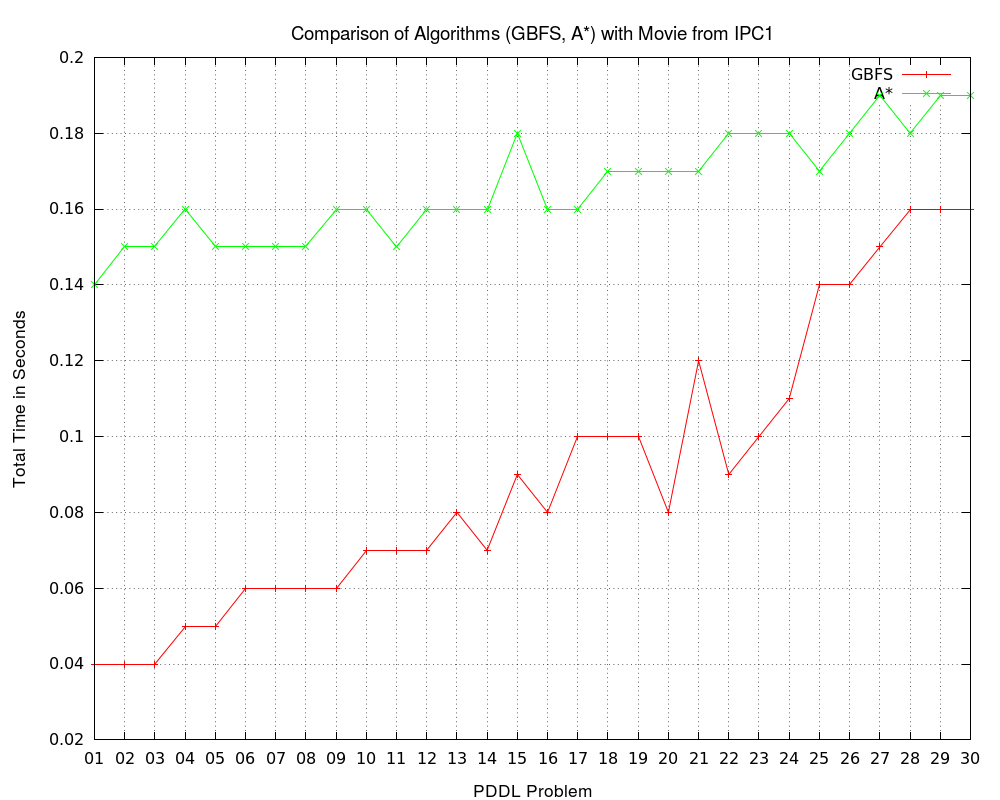
\includegraphics[scale=0.35]{MovieTime.png}
    \caption{Movie domain from IPC1, GBFS + EHC vs A* }
    \label{fig:MovieDomainTime}
\end{figure} 

The Movie domain has always the same goal, i.e. to get lots of snacks before watching the movie. The planners finish when all the snacks set out in the problem have been accumulated as well as the success of all other parameters set out in the problem. Each problem requires ADL, as discussed in Chapter \ref{Chapter2}. The problems for both planners are relatively easy but in terms of speed at achieving the goal, the new algorithm fairs better in every problem than A*. You can see from the graph (GBFS with EHC red, A* green) that the paths of the lines never cross or are even close to each other. Along the X axis is the time in seconds, the Y axis has the number of problems. We can see that the new algorithm as well as A* had a steady increase in line with the increase in difficulty of the problem and the time taken to solve them but even then, the times are not similar. From the raw data that can be accessed from the information in Appendix A, EHC failed for every problem but GBFS with EHC was still able to complete each problem faster than A*.
\\
\begin{figure}[!htb]
    \centering
    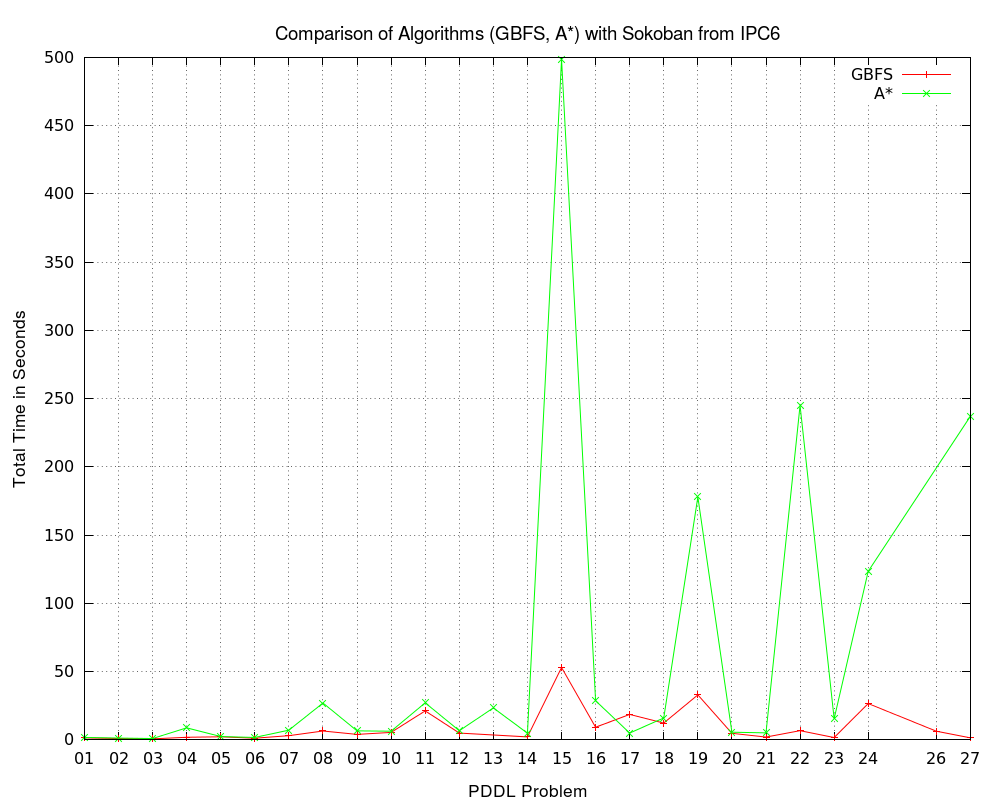
\includegraphics[scale=0.35]{SokobanTime.png}
    \caption{Sokoban domain from IPC6, GBFS + EHC vs A* }
    \label{fig:SokobanDomainTime}
\end{figure}
Let's look at the Sokoban domain which was used for the IPC6 competition. Sokoban is a game where there are crates in certain locations and the goal is to take one crate at time from the starting point to an end point but being careful not to block yourself in or get stuck. 
The domain has a total of 30 problems but both algorithms could only solve 25 each, however, the results regarding time are mostly better for GBFS with EHC.  From the graph it is clear that GBFS with EHC was able to solve the same number of problems but in a faster time; with some of the problems, the time taken is relatively close but in others there is a huge difference.    
\\
\begin{figure}[!htb]
    \centering
    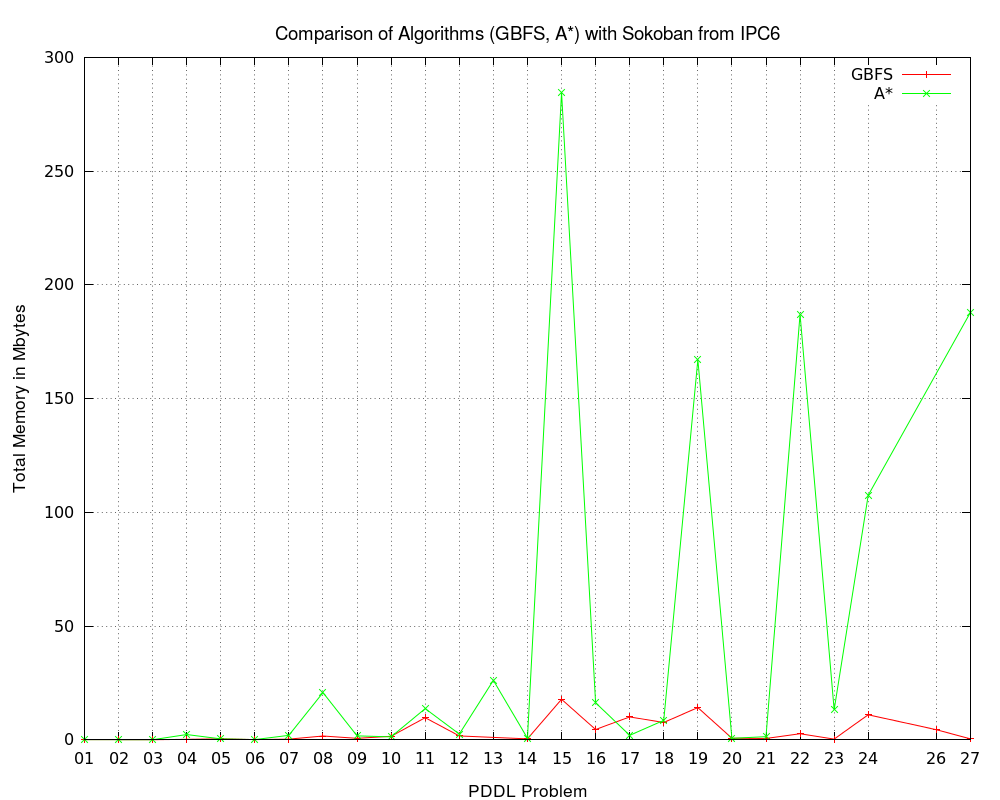
\includegraphics[scale=0.35]{SokobanMemory.png}
    \caption{Sokoban domain from IPC6, GBFS + EHC vs A* }
    \label{fig:SokobanDomainMemory}
\end{figure} 
Looking at the results on memory consumption for both A* and GBFS with EHC in the Sokoban domain, Figure \ref{fig:SokobanDomainMemory} shows that an increase in time yields an increase in memory consumption with the largest disparity showing up in problem 15. Here, GBFS with EHC was able to solve the problem in 52.99 seconds and use 17.82Mbytes of memory, whereas A* took 496.38 seconds and used 284.31 Mbytes, which is a difference of 443.39 seconds and 266.49Mbytes. To put this in perspective, GBFS with EHC would need to solve problem 15 in Sokoban 15 times in order to match the same memory consumption used by A*. 
Earlier in Chapter \ref{Chapter4}, we presented results of a preliminary test in the Blocksworld domain, showing the speed of GBFS with EHC.  Now, within the same domain, we will look at the memory usage for problems 01-35 (see Figure \ref{fig:BlocksworldDomainMemory}).
\\
\begin{figure}[!htb]
    \centering
    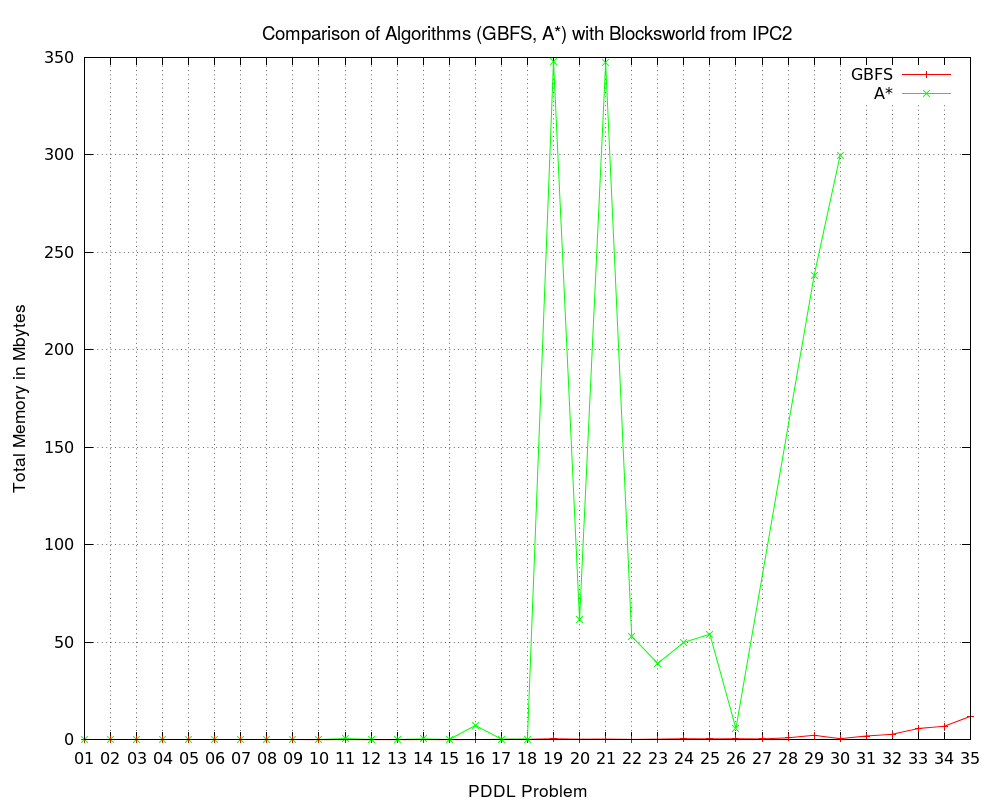
\includegraphics[scale=0.35]{BlocksworldMemory.png}
    \caption{Blocksworld domain from IPC2, GBFS + EHC vs A* }
    \label{fig:BlocksworldDomainMemory}
\end{figure}
From the graph we can see a very slow, steady increase in memory usage as the plans become more complicated for the GBFS with EHC algorithm, however, for the A* algorithm, things were more complicated. The maximum memory used by GBFS with EHC was done so when solving the hardest problem in the domain, i.e. 12.05Mbytes was used by GBFS with EHC for problem 35. If we look at the maximum memory used by A*, it was 348.12Mbytes and 347.07 Mbytes for problems 19 and 21 respectively, neither of which are the hardest problem. As well as this, we can also see that A* was unable to complete Blocksworld problems 31-35.
\begin{figure}[!htb]
    \centering
    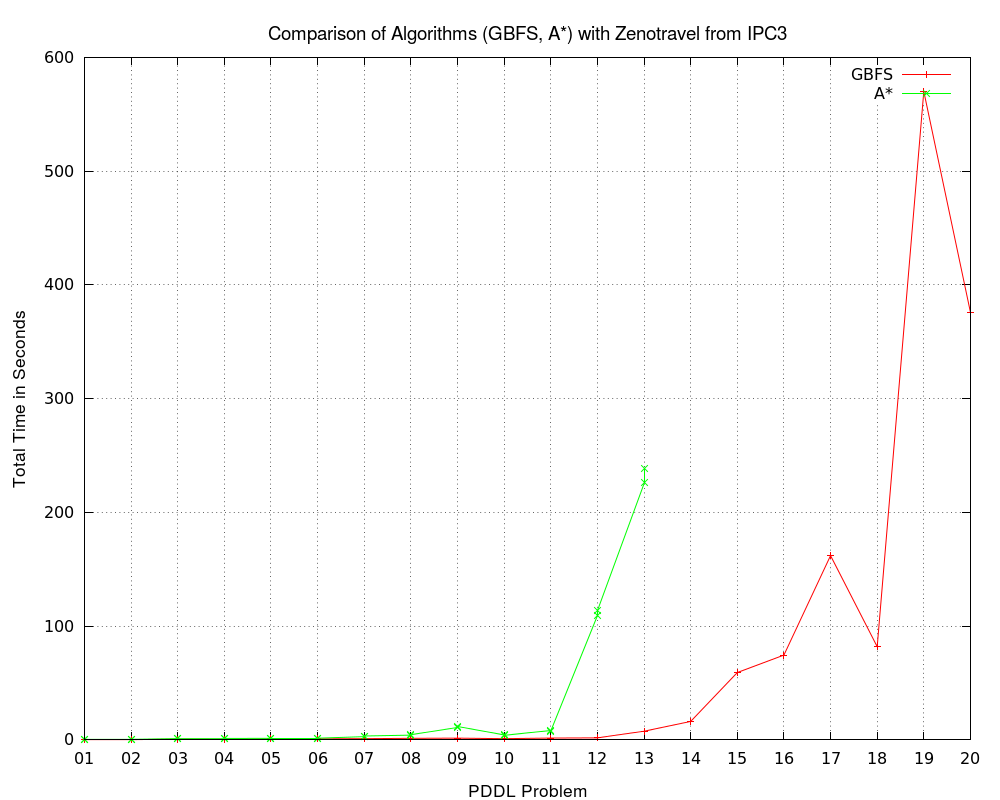
\includegraphics[scale=0.35]{ZenoTime.png}
    \caption{Zenotravel domain from IPC3, GBFS + EHC vs A* }
    \label{fig:ZenoTravelDomainTime}
\end{figure}
\\
If we look at Zenotravel from IPC3 Figure\ref{fig:ZenoTravelDomainTime}, GBFS with EHC was able to solve all 20 of the problems within the domain, but A* was only able to solve 13. The time gradually increases as the problems get harder in the domain for both algorithms but for GBFS with EHC there is a huge increase of time from problem 18 to 19. This could be because of the increase of facts, as problem 18 has 585 facts whilst problem 19 has 760. Also in problem 17 there is a total number of 16880 possible action which increases to 20970 in problem 18, then 19 has an even bigger increase to 26500. This increase could be the reason why the time has dramatically risen. 
\begin{figure}[!htb]
    \centering
    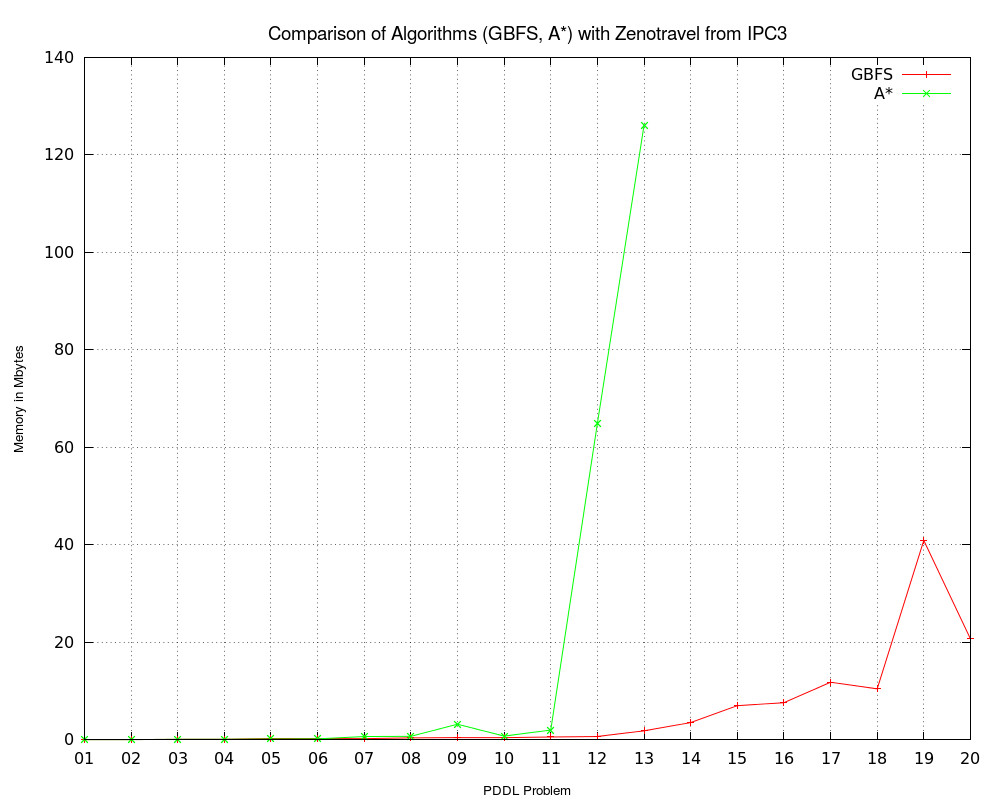
\includegraphics[scale=0.35]{ZenoMemory.png}
    \caption{Zenotravel domain from IPC3, GBFS + EHC vs A* }
    \label{fig:ZenoTravelDomainMemory}
\end{figure}
Then in contrast in Figure\ref{fig:ZenoTravelDomainMemory}, as the problems get harder, the memory consumption usually goes up along with it, which is what happened to A* but GBFS with EHC kept a steady increase of memory consumption with a small spike at problem 19. We can see by all the graphs shown that in terms of speed and memory consumption, GBFS with EHC is dominantly better.
\subsection{Null Plans}
Even though a preprocessing test was carried out for all domains, there were some that did not parse correctly and further analysing of these tests showed that some of the domains did not work correctly or there was issues with them which made it impossible for the planners to even attempt the domains. We can see automatically which domains or problems had potential problems as both of the planners were unable to solve any of the problems and the text files pertaining to the problem output were empty. To name one, the Barman domain was unable to be parsed correctly and that is why each of the algorithms have 0 solved problems.
\subsection{Validity}
As discussed in Chapter \ref{Chapter3}, we used VAL\cite{VAL} to check the new search algorithm to ensure that it was providing logically sound plans. As there were over 1000 tests, we selected a few problems to test using VAL. We felt that if these 5 tests came back positive then the algorithm was able to produce logically sound plans for all domains as we have a mix of STRIPS and ADL as well as easy, medium and hard problems. 
The 5 problems selected were:
\begin{itemize}
\item Problem 1 from PSR
\item Problem 10 from Zenotravel
\item Problem 20 from Blocksworld
\item Problem 01 from Sokoban
\item Problem 10 from Blocksworld
\end{itemize} 
All 5 of the tests came back positive and all 5 were valid. As there we no errors in any of the plans, we can assume that all plans will be valid from the new search algorithm.  
All raw data files can be found in Appendix B.
\section{$H^m$ vs Fast Forward vs Max vs Sum}
For comparison with regards to heuristics, we used the same search algorithm (A*) with all 4 of the heuristics. We tested them with the same script and same set of problems. As before, each problem was capped at 600 seconds to solve a problem. The results gained were not as good as the search algorithm and in terms of solved problems it was worse than expected. The $H^m$ heuristic was unable to solve more problems than any of the other 3 heuristics but we assumed this could happen as it is costly to generate all subsets of a problem. Because of this, the $H^m$ heuristic was only able to solve 12 of the Blocksworld problems within the 600-second time limit. The two admissible heuristics ($H^m$ and Max) performed worse in the Blocksworld domain. Max was only able to solve 6 more problems than $H^m$ but FF and Sum solved nearly all problems (see Figure \ref{BlocksworldDomainHeuristicCompare}). 
\begin{figure}[!htb]
    \centering
    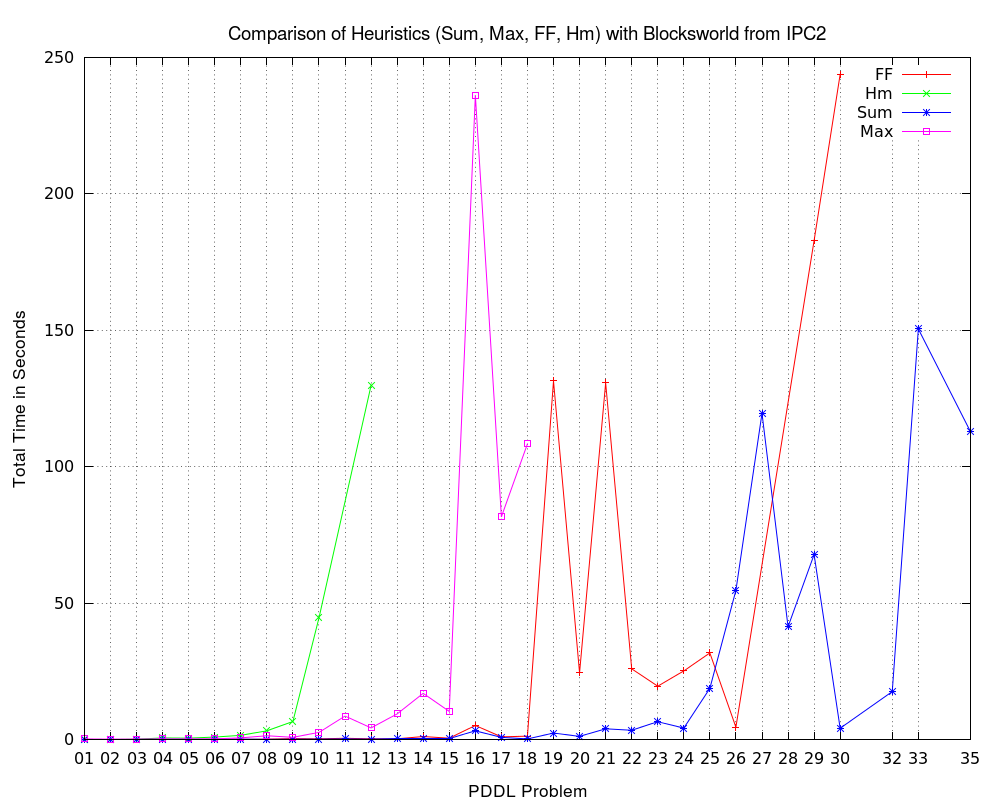
\includegraphics[scale=0.35]{BlocksworldTimeHeuristics.png}
    \caption{Blocksworld domain from IPC2, Sum vs FF vs Max vs $H^m$}
    \label{fig:BlocksworldDomainHeuristicCompare}
\end{figure}
If we then take a look at the Movie domain from IPC1 (see Figure \ref{fig:MovieTotalTimeHeuristics}, $H^m$ was able to solve all 30 problems, as could the other 3 heuristics. $H^m$ was a little slower than the other 3 in solving the problems but was able to do it within the 600-second time limit. Again, the not admissible heuristics proved to be better in terms of time within this domain. The memory consumption of each of the heuristics was exactly the same except for Sum being more efficient towards the end.
\begin{figure}[!htb]
    \centering
    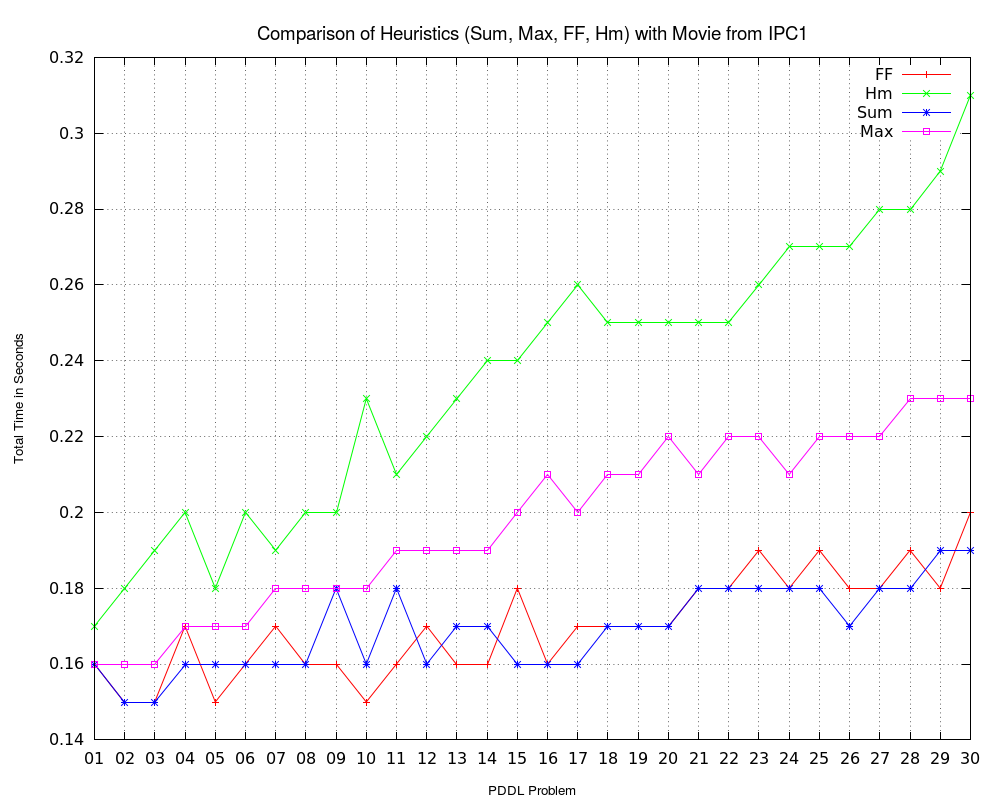
\includegraphics[scale=0.35]{MovieTotalTime.png}
    \caption{Movie domain from IPC1, Sum vs FF vs Max vs $H^m$}
    \label{fig:MovieTotalTimeHeuristics}
\end{figure}
The last strange result is that the plan size for all 4 heuristics was the same for each problem. Even though the Movie domain has many small problems, every problem having the same plan size for not admissible and admissible heuristics is not what we expected (see Figure \ref{fig:MoviePlanSize}). 
\begin{figure}[!htb]
    \centering
    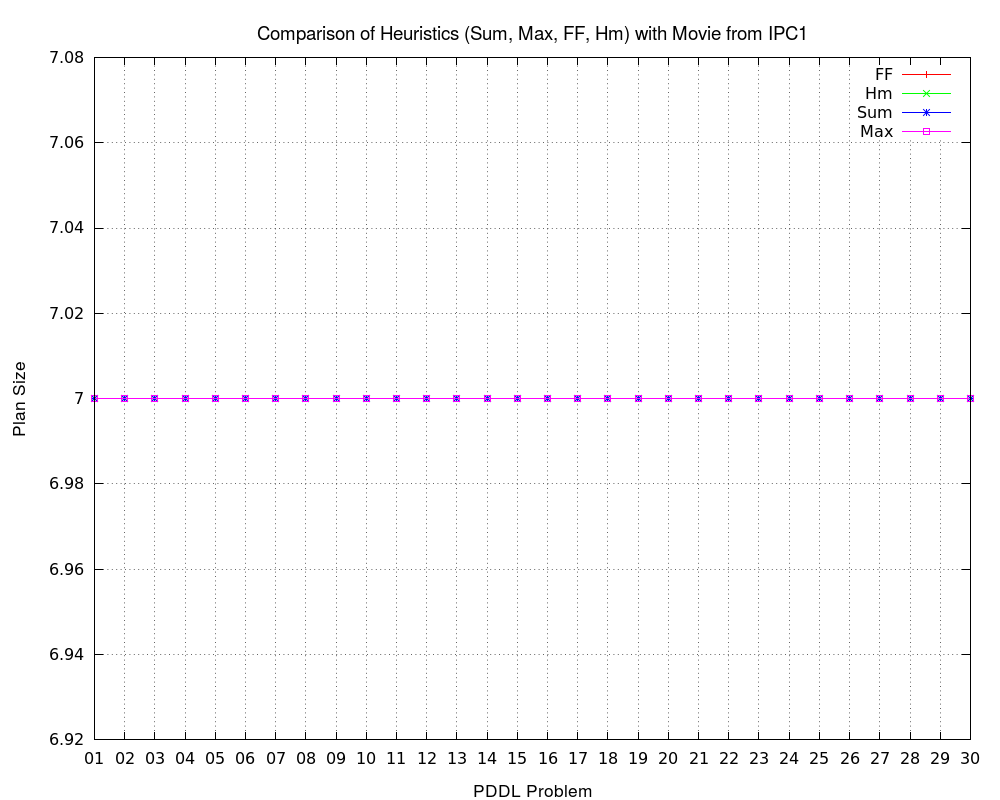
\includegraphics[scale=0.35]{MoviePlanSize.png}
    \caption{Movie domain from IPC1, Sum vs FF vs Max vs $H^m$}
    \label{fig:MoviePlanSize}
\end{figure}
As stated in \cite{HmHeuristic} the $H^m$ heuristic exhausts memory and this was the case multiple times during testing. Within a lot of the domains, the heuristic failed to solve any problems and memory was exhausted, that being said, within some of the domains compared to an admissible heuristic like Max, the results were similar in terms of solved problems but it was still the worse of the three. In some of the domains like Freecell, the $H^m$ heuristic was unable to solve any of the problems. 
What we saw was within the Blocksworld domain, there were anomalies between admissible and non admissible heuristic in terms of actions used to achieve a goal. 
%INSERT PICTURE!!!!!!!!
Above are the actions used to complete the Blocksworld problem 4 for all 4 heuristics. With regards to the two admissible heuristics $H^m$ and Max, we can see some differences in the actions used to complete the problem. At step \textit{02} the $H^m$ heuristic guided the algorithm to pick up block d whilst Max unstacked e b. Fast Forward and Sum did the same action at this stage. Even though all plan sizes are the same in length, these steps can describe a more critical path to the goal from the starting node. 
\section{SAT4J}
We wanted to test to see how a satisfiability planner solved PDDL problems. Even though there are a lot of SAT planners\cite{BlackBox}\cite{SATPLAN} we decided to take a Blocksworld problems and encode them to SAT problems within the PDDL4J library, then give the output to a SAT solver (in this case SAT4J) and see how much of a difference there was in terms of speed at solving satisfiability problems. We encoded 9 PDDL problems from the Blocksworld domain (p01-p09) and provided the files to SAT4J. 
We discovered that SAT4J was able to complete Blocksworld problem 9 within 0.037 seconds. Compared to A* which was 0.82 seconds and GBFS with EHC was 0.10 seconds. It shows that using a SAT solver is nearly 10x faster at solving problems. 
\begin{verbatim}
c org.sat4j.minisat.constraints.cnf.OriginalBinaryClause => 4
c org.sat4j.minisat.constraints.cnf.OriginalWLClause => 13
c ignored satisfied constraints => 17
c 34 constraints processed.
s SATISFIABLE
v -1 2 -3 -4 -5 -6 -7 -8 0
c Total wall clock time (in seconds) : 0.037
\end{verbatim}
Due to time constraints, only the Blocksworld domain was tested. With more time, we could test all of the IPC domains for a comparable analysis. 
\section{GBFS with $H^m$}
We combined the new search algorithm with the new heuristic to see if the plan size would be smaller when using a heuristic that should provide the optimal path. When the problems became harder, the GBFS with EHC + FF plan size grew but when applied with $H^m$, the plan size was considerably smaller as you can see from Figure \ref{fig:BlocksworldDomainGBFSwithHm}.
\begin{figure}[!htb]
    \centering
    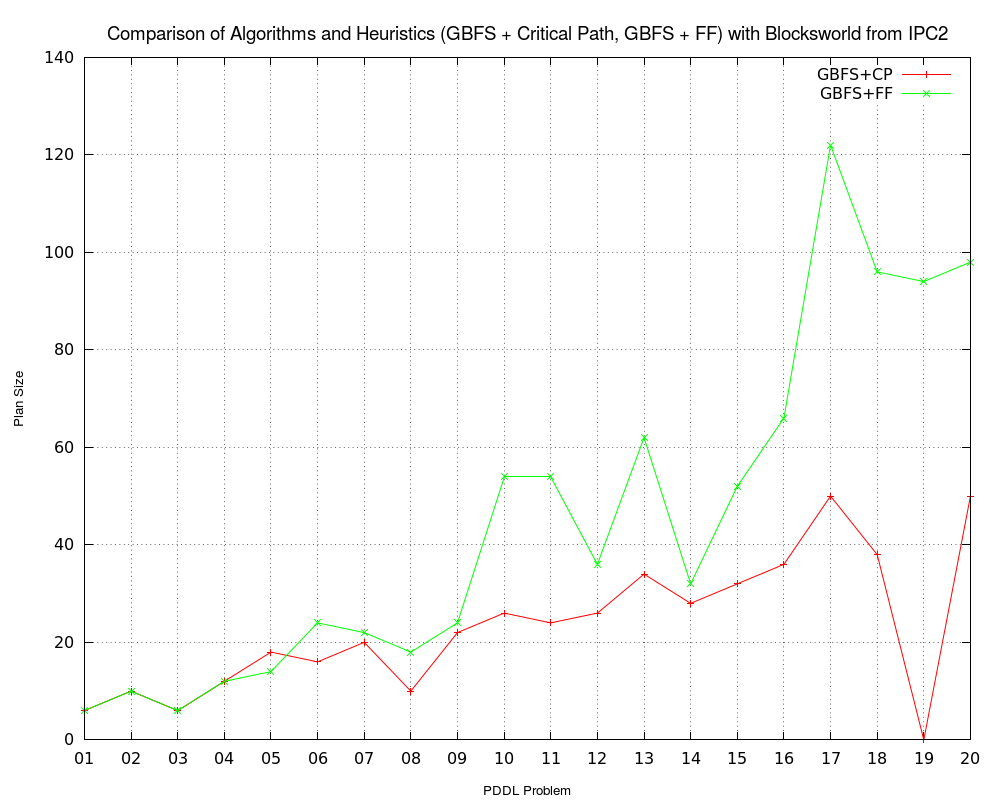
\includegraphics[scale=0.35]{BlocksworldPlanSizeGwithCP.png}
    \caption{Blocksworld domain from IPC2, GBFS with EHC + FF vs GBFS + $H^m$ }
    \label{fig:BlocksworldDomainGBFSwithHm}
\end{figure}
As the $H^m$ heuristic was only able to complete 19 out of the 35 problems within the time limit, we selected only the first 20 problems to create the graph \ref{fig:BlocksworldDomainGBFSwithHm}. Except for one instance (PDDL problem 5), the $H^m$ heuristic plan size stayed below GBFS with EHC using Fast Forward. As $H^m$ is an admissible heuristic it provided a better quality plan as it did not overestimate or under-estimate the distance from the starting node to the goal node.  
This was a good result for the Blocksworld problem but applying the same approach to Elevator from IPC2 did not provide the same set of results. 
\begin{figure}[!htb]
    \centering
    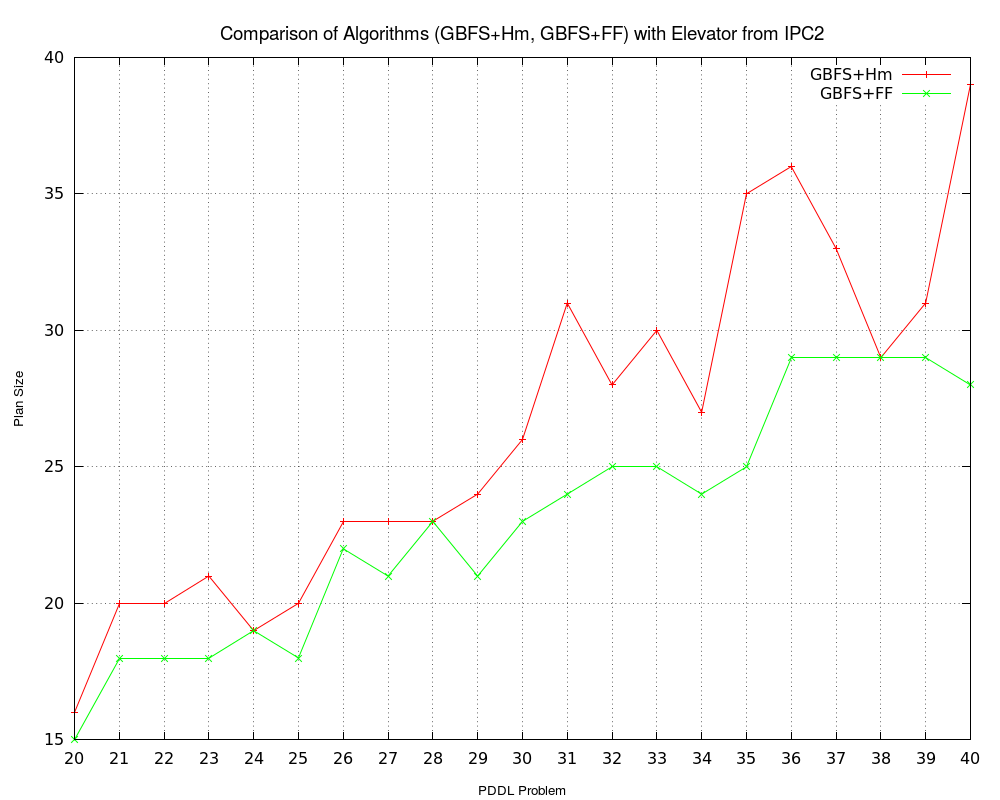
\includegraphics[scale=0.35]{Elevator20to40PlanSize.png}
    \caption{Elevator domain from IPC2, GBFS + FF vs GBFS + $H^m$ }
    \label{fig:ElevatorDomainGBFSwithHm}
\end{figure}
We can see that with some of problems, the plan size was the same but with the majority of others the plan size for $H^m$ was larger which is not what we expected given the results from the Blocksworld domain. 
\section{Test of Hypotheses}
In Chapter \ref{Chapter2}, we made hypotheses about the new search algorithm (GBFS with EHC) and the new heuristic $H^m$. With regards to the search algorithm, we devised the hypothesis that it would able to solve more problems than the current algorithm (A*). From the final results, we can say that this hypothesis is now true, as GBFS with EHC was able to solve 21 more problems than A*. It is a small number in the grand scheme of how many problems were tested but it proves that the current algorithm is not better in terms of solved problems. 
We also stated that the new algorithm would be faster and use less memory than A*. From the results presented within this chapter and the raw data, we can safely say that this is true. The results in certain domains were close but in others GBFS with EHC proved to be the more superior algorithm for classical planning.
With the new heuristic we saw that it was unable to complete more problems than the other heuristics within the library and also the speed and memory consumption was not better overall. We were able to spot some anomalies within the actions used to achieve a goal from the Blocksworld domain which suggest that the other heuristics are not using the most optimal approach when solving a problem. This concerns Max more as it is an admissible heuristic, even though it does not overestimate or under-estimate the distance to the goal, it uses actions that are possibly more costly in achieving a goal. 